\chapter{Architektura systemu}

Założeniem projektu było stworzenie algorytmu weryfikacji modelowej w oparciu o własności LTL dla języka Alvis w środowisku rozproszonym.

Alvis to język formalny, którego celem jest dostarczenie elastyczności w modelowaniu systemów współbieżnych i czasu rzeczywistego wraz z możliwością weryfikacji opartej o metody formalne.
Stanowi połączenie zalet języków wysokiego poziomu z graficznym budowaniem zależności między podsystemami (nazywanymi agentami).
% TODO jak dużo o Alvisie takiego wstępu?


\section{System rozproszony}

Architektura systemu została zaplanowana tak, aby wydzielić funkcjonalności do odseparowanych aplikacji.
Całość składa się z 3 programów oraz bazy danych.
Jej schemat ogólny został przedstawiony na rys. \ref{fig:system_overview}.

\begin{figure}[h]
    \centering
    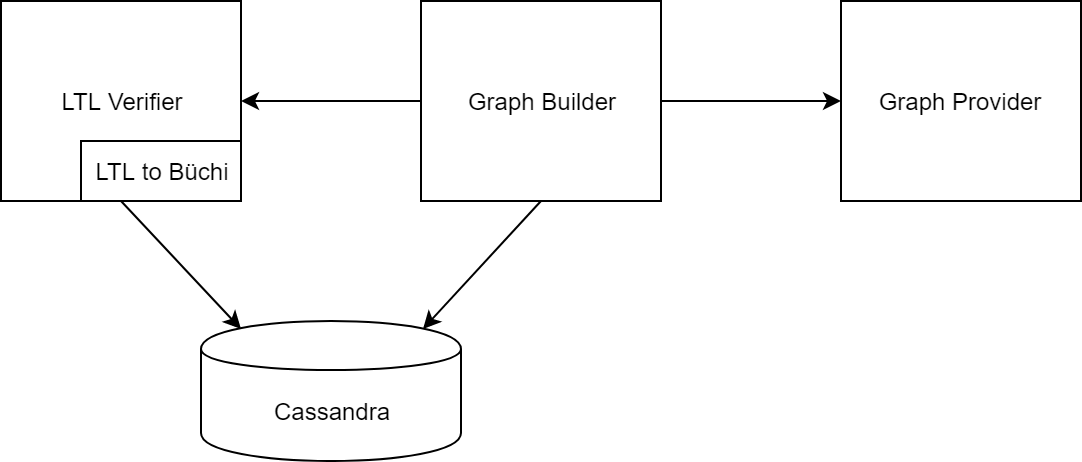
\includegraphics[width=\linewidth,keepaspectratio]{img/system_overview.png}
    \caption{Schemat ogólny systemu.}
    \label{fig:system_overview}
\end{figure}

Pierwszym elementem jest \textit{Graph Provider} (\textbf{GP}).
Spełnia on dwa zadania.
Pierwsze z nich to dostarczanie wszystkich osiągalnych tranzycji dla danego stanu.
Drugie umożliwia otrzymanie stanów dla zadanej tranzycji, które można odwiedzić z wybranego stanu źródłowego.
Serwis ten enkapsuluje działanie całej domeny.
Jako jedyny dostarcza dane, dzięki którym da się zbudować całą przestrzeń stanów.
GP spełnia prosty interfejs przedstawiony w listingu \ref{lst:graph_provider_interface}.

\begin{lstlisting}[caption={Interfejs implementowany przez GP.},captionpos=b,label={lst:graph_provider_interface}]

  public interface GraphProvider {
    Collection<Transition> allTransitionFromState(SystemState from);

    Collection<SystemState> allReachableStates(SystemState from,
                                               Transition through);
  }
\end{lstlisting}

\textit{LTL Verifier} (\textbf{LV}) to główna serwerowa aplikacja zajmująca się weryfikacją modelową i zawiera główną część tego algorytmu.
Konwertuje ona także formuły LTL do automatów Büchiego.
Napisana została w języku Java z wykorzystaniem frameworka Spring.
Interfejs implementowany przez LV opisuje listing \ref{lst:ltl_verifier_interface}.

\begin{lstlisting}[caption={Interfejs implementowany przez LV.},captionpos=b,label={lst:ltl_verifier_interface}]

  public interface LtlVerifier {
    VerificationId createVerificationJob(VerificationInit verificationInit);

    VerificationResult newStates(NewStates newStates,
                                 VerificationId id);

    VerificationResult finish(VerificationId id);
  }
\end{lstlisting}

\textit{Graph Builder} (\textbf{GB}) spełnia rolę serca systemu.
To centrum sterowania, które inicjuje zapytania do pozostałych aplikacji.
Zarządza eksploracją kolejnych stanów, a także wysyła je do weryfikacji.
Zarówno GB jak i LV komunikują się z bazą danych (Cassandra), aby czytać i zapisywać stany czy tranzycje.
Komunikacja między GB a GP zachodzi za pomocą Apache Thrift, wykorzystując binarny protokół przesyłając dane siecią.
Zapytania GB do LV realizowane są poprzez protokół HTTP w formacie JSON.

% TODO dopisać o celach i możliwościach architektury, może diagram z wyszczególnionymi protokołami komunikacji
